% Following figures are from /Users/zang/Desktop/fit_results/fit_taunub_sys_1l_allVR_BONLY_MU3000_gU2_5_23L1_0_noWeights_N_minus_1_fullRegion_v3_HEPData/Plots/
% Source files: topCR_1tau1e_Res*_postFit.eps and topCR_1tau1e_Res*_postfit.yaml.
% Local verified copies: data/ch8/hepdata_20260924/ (Plots, Histograms, Fits).
% Styling: scripts/ch8/restyle_hepdata.py; native data and ratio drawings are preserved.
% Verification: output/ch8/hepdata_update_20260924/figures.json.
% Axis notation/font update: scripts/ch8/axis_labels.py; output/ch8/axis_labels_20260924/.
% Previous version: figures_topcr_bonly_20260921.tex (selected by \CHEightCRFigureVersion).
\begin{figure}[htpb]
    \centering
    \begin{subfigure}{0.49\linewidth}
        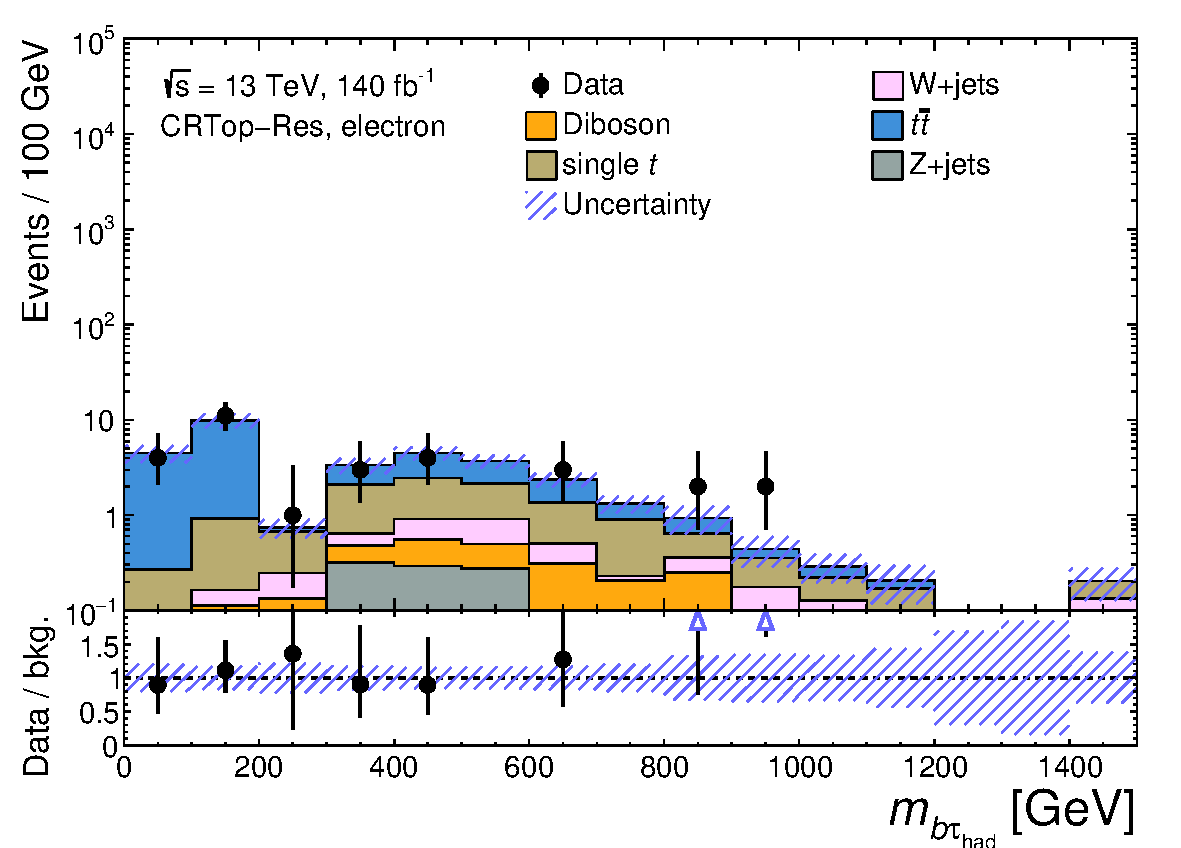
\includegraphics[width=\linewidth]{Figs/CH8/hepdata/topCR_1tau1e_Res_InvM_N_minus_1_Mtaub.pdf}
        \caption[]{$m_{b\hadtau}$}
    \end{subfigure}\hfill
    \begin{subfigure}{0.49\linewidth}
        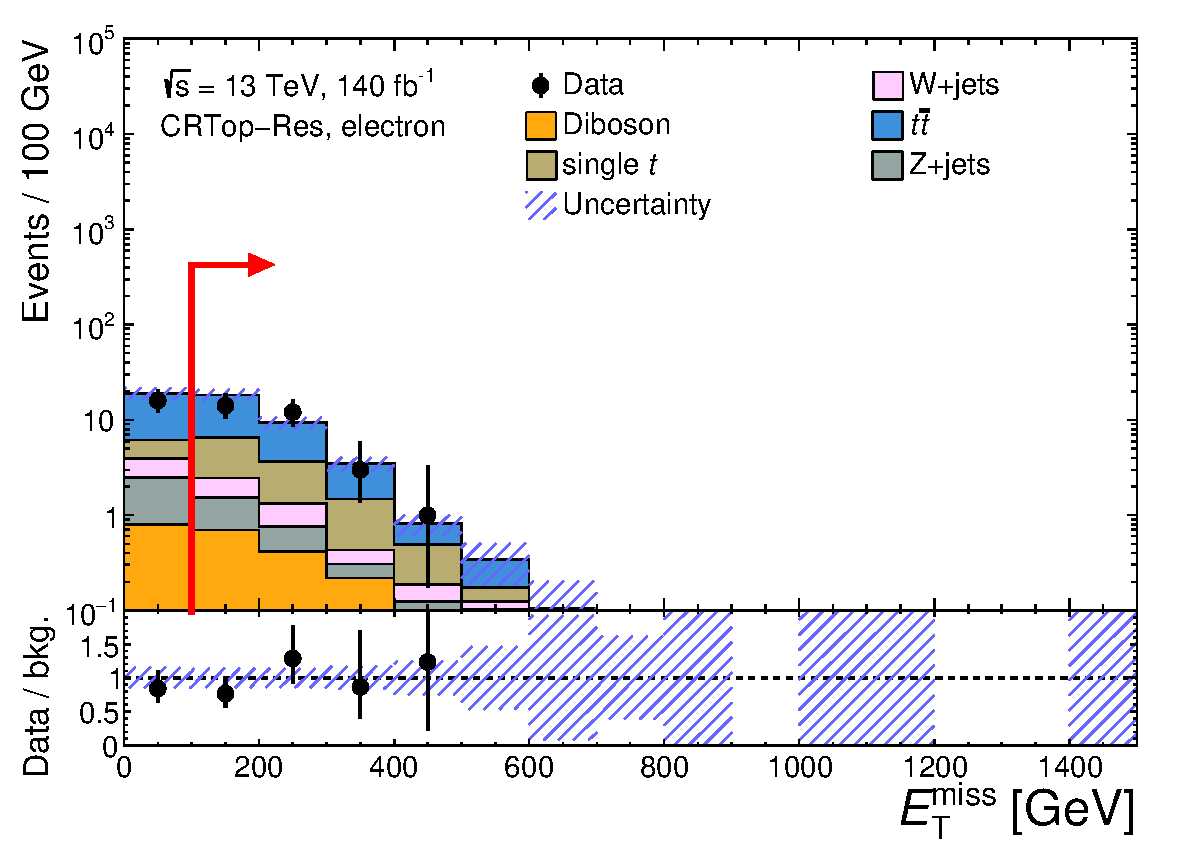
\includegraphics[width=\linewidth]{Figs/CH8/hepdata/topCR_1tau1e_Res_met_N_minus_1_met.pdf}
        \caption[]{$\met$}
    \end{subfigure}\\
    \begin{subfigure}{0.49\linewidth}
        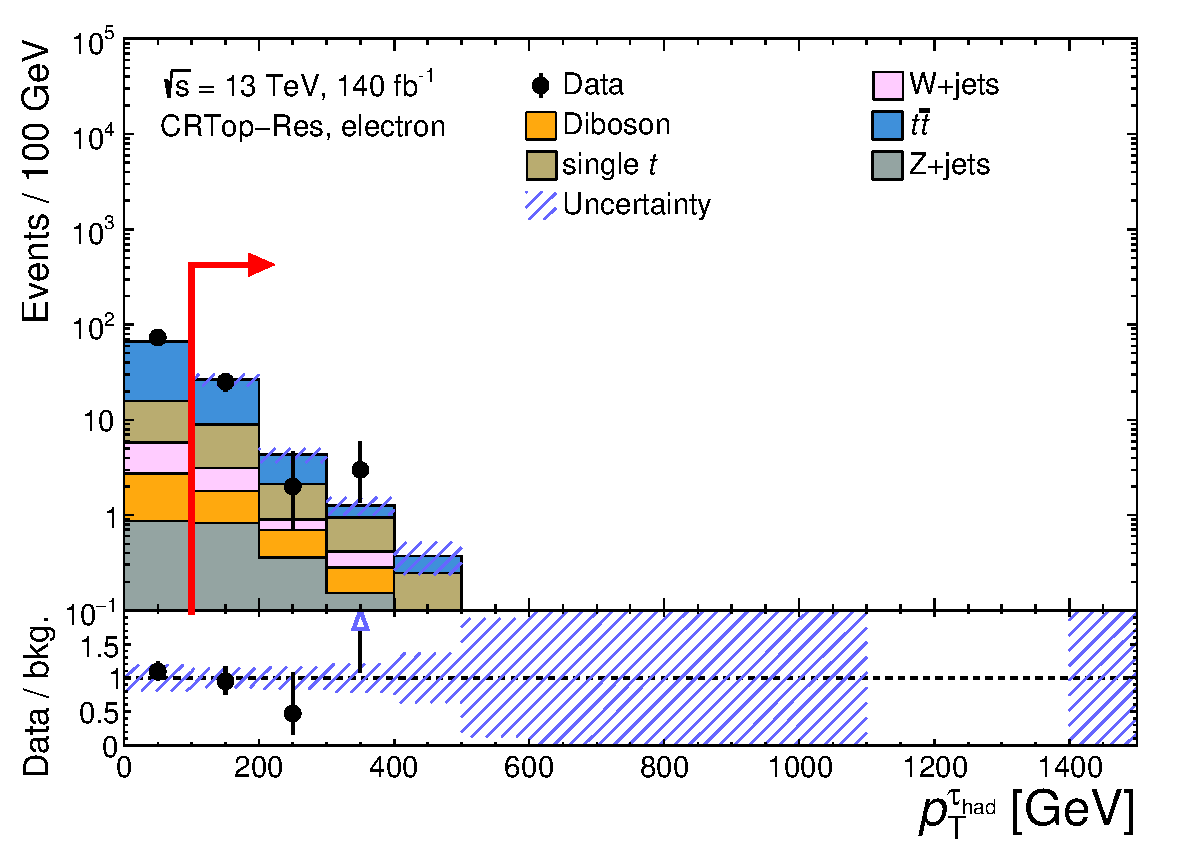
\includegraphics[width=\linewidth]{Figs/CH8/hepdata/topCR_1tau1e_Res_tau_pT_N_minus_1_tau_pt_0.pdf}
        \caption[]{$\pT^{\hadtau}$}
    \end{subfigure}\hfill
    \begin{subfigure}{0.49\linewidth}
        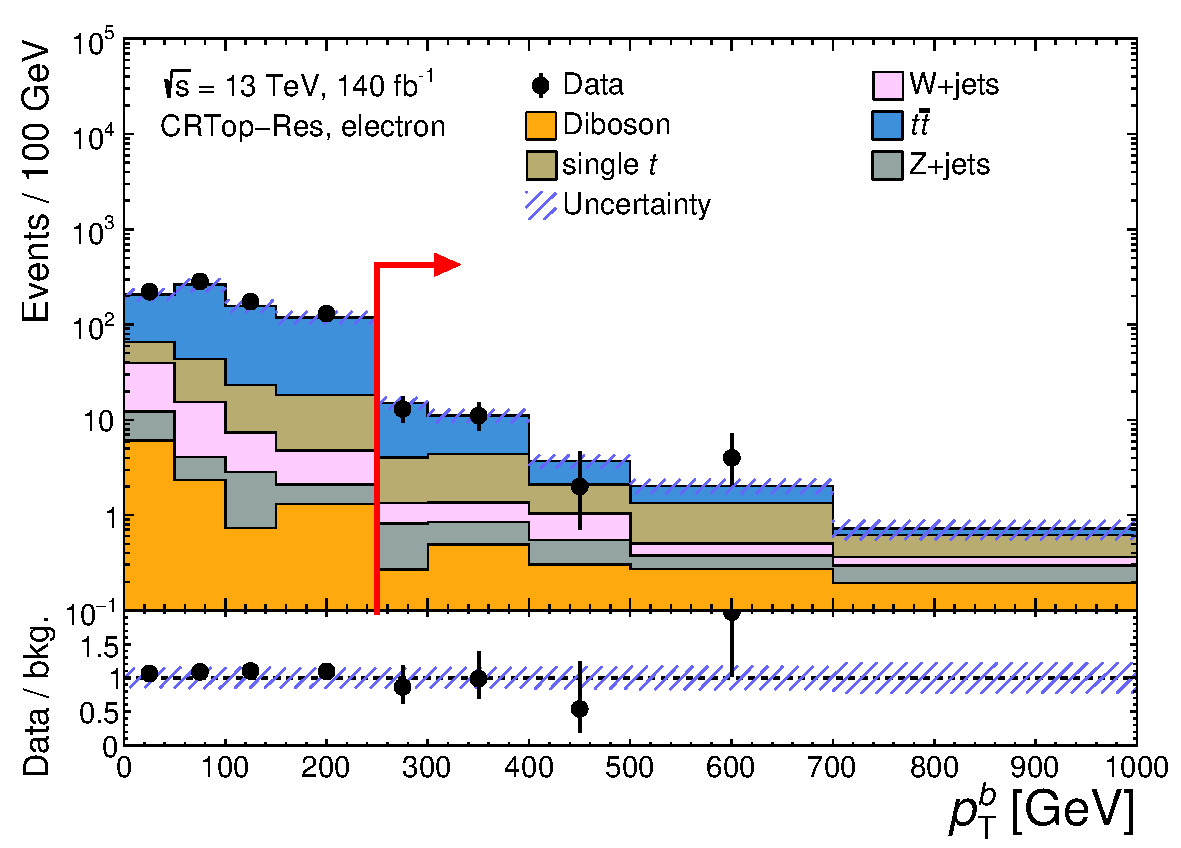
\includegraphics[width=\linewidth]{Figs/CH8/hepdata/topCR_1tau1e_Res_bJet_pT_0_N_minus_1_bjet_pt_0.pdf}
        \caption[]{$\pT^b$}
    \end{subfigure}
% Other N-1 panels retained for reference; temporarily hidden.
%     \begin{subfigure}{0.49\linewidth}
%         \includegraphics[width=\linewidth]{Figs/CH8/hepdata/topCR_1tau1e_Res_mT_N_minus_1_mT_tau_met.pdf}
%         \caption[]{$\mT$}
%     \end{subfigure}\hfill
%     \begin{subfigure}{0.49\linewidth}
%         \includegraphics[width=\linewidth]{Figs/CH8/hepdata/topCR_1tau1e_Res_n_bjets_N_minus_1_n_bjets.pdf}
%         \caption[]{$N_b$}
%     \end{subfigure}
    \caption[Background-only fit distributions in CRTop-Res, electron channel]{$N-1$ distributions in $\CRTop$-$\Res$ for the $e$ channel after the background-only fit. The hatched bands show the combined statistical and systematic uncertainties. The bottom panels show the ratio of data to background prediction. Red arrows indicate variable thresholds for the $\CRTop$ regions. The last bin includes overflow.}
    \label{fig:ch8_topcr_res_e}
\end{figure}

% Following figures are from /Users/zang/Desktop/fit_results/fit_taunub_sys_1l_allVR_BONLY_MU3000_gU2_5_23L1_0_noWeights_N_minus_1_fullRegion_v3_HEPData/Plots/
% Source files: topCR_1tau1mu_Res*_postFit.eps and topCR_1tau1mu_Res*_postfit.yaml.
% Local verified copies: data/ch8/hepdata_20260924/ (Plots, Histograms, Fits).
% Styling: scripts/ch8/restyle_hepdata.py; native data and ratio drawings are preserved.
% Verification: output/ch8/hepdata_update_20260924/figures.json.
% Axis notation/font update: scripts/ch8/axis_labels.py; output/ch8/axis_labels_20260924/.
% Previous version: figures_topcr_bonly_20260921.tex (selected by \CHEightCRFigureVersion).
\begin{figure}[htpb]
    \centering
    \begin{subfigure}{0.49\linewidth}
        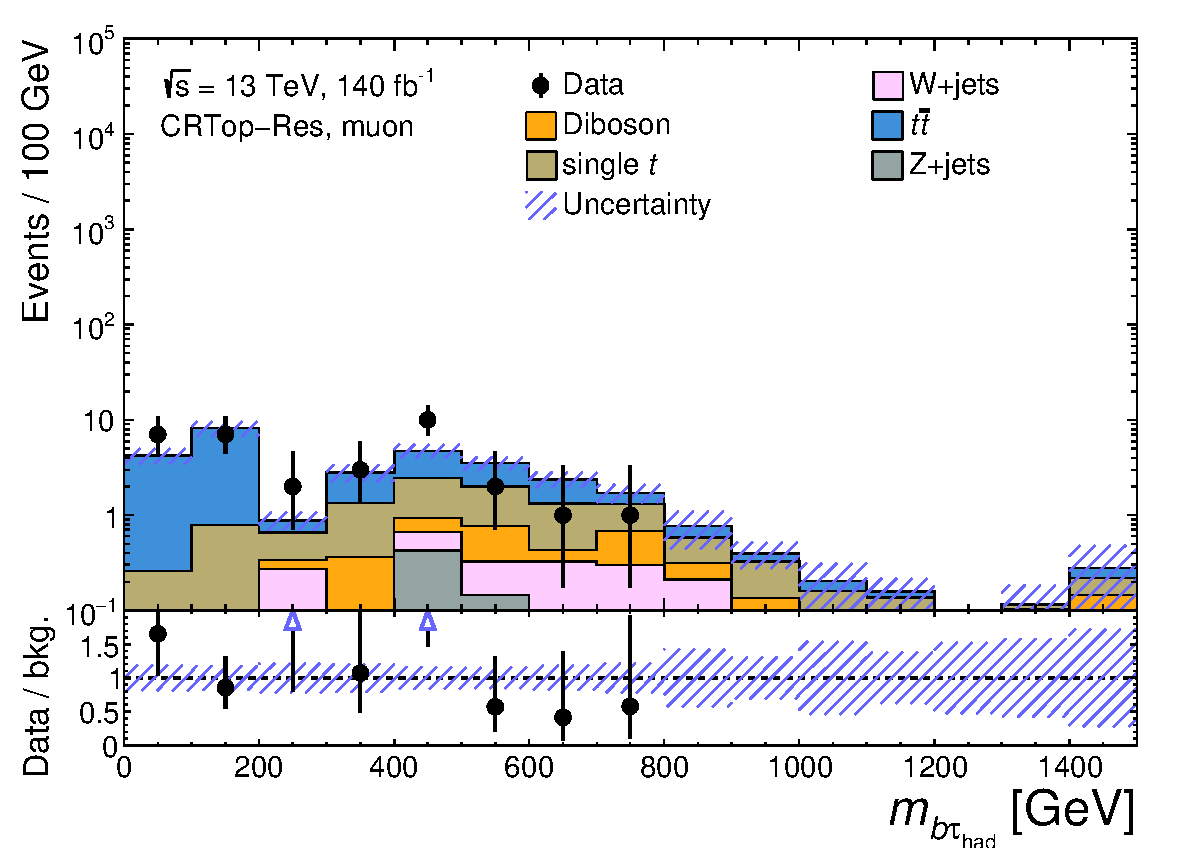
\includegraphics[width=\linewidth]{Figs/CH8/hepdata/topCR_1tau1mu_Res_InvM_N_minus_1_Mtaub.pdf}
        \caption[]{$m_{b\hadtau}$}
    \end{subfigure}\hfill
    \begin{subfigure}{0.49\linewidth}
        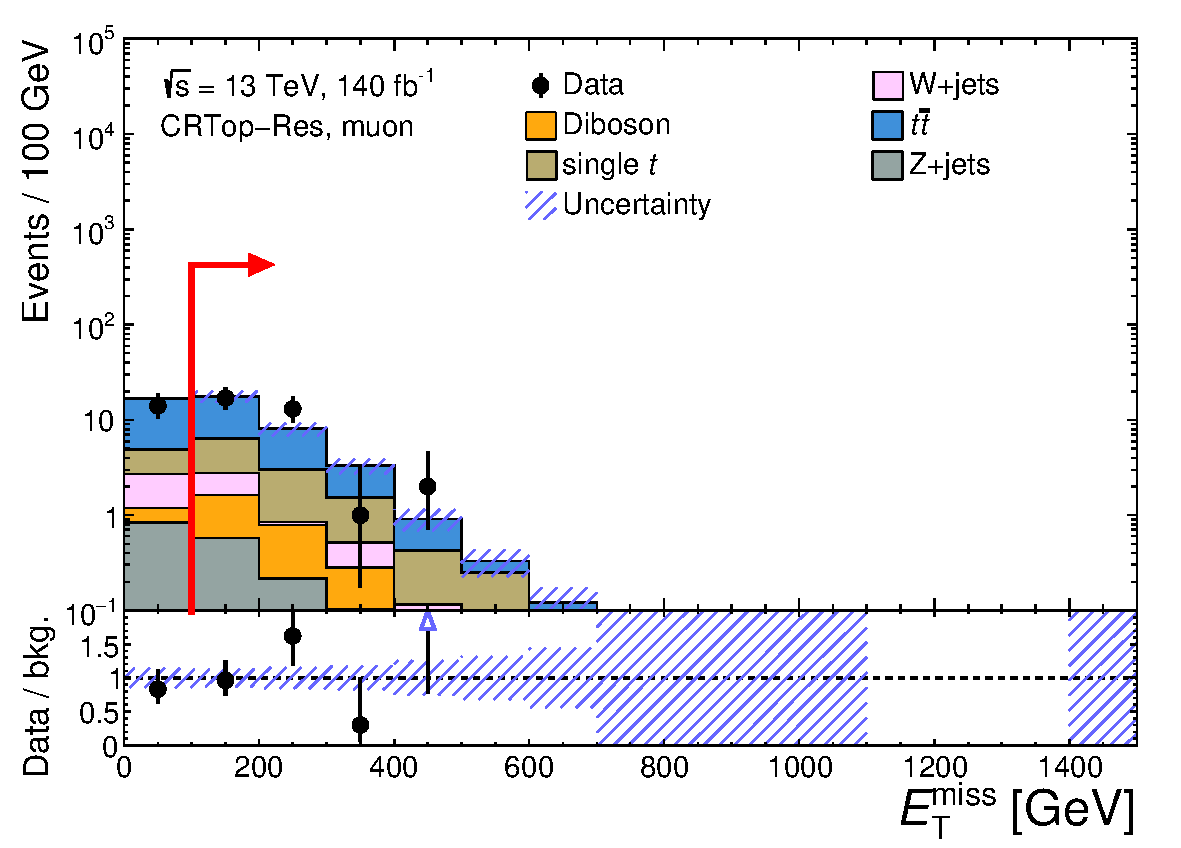
\includegraphics[width=\linewidth]{Figs/CH8/hepdata/topCR_1tau1mu_Res_met_N_minus_1_met.pdf}
        \caption[]{$\met$}
    \end{subfigure}\\
    \begin{subfigure}{0.49\linewidth}
        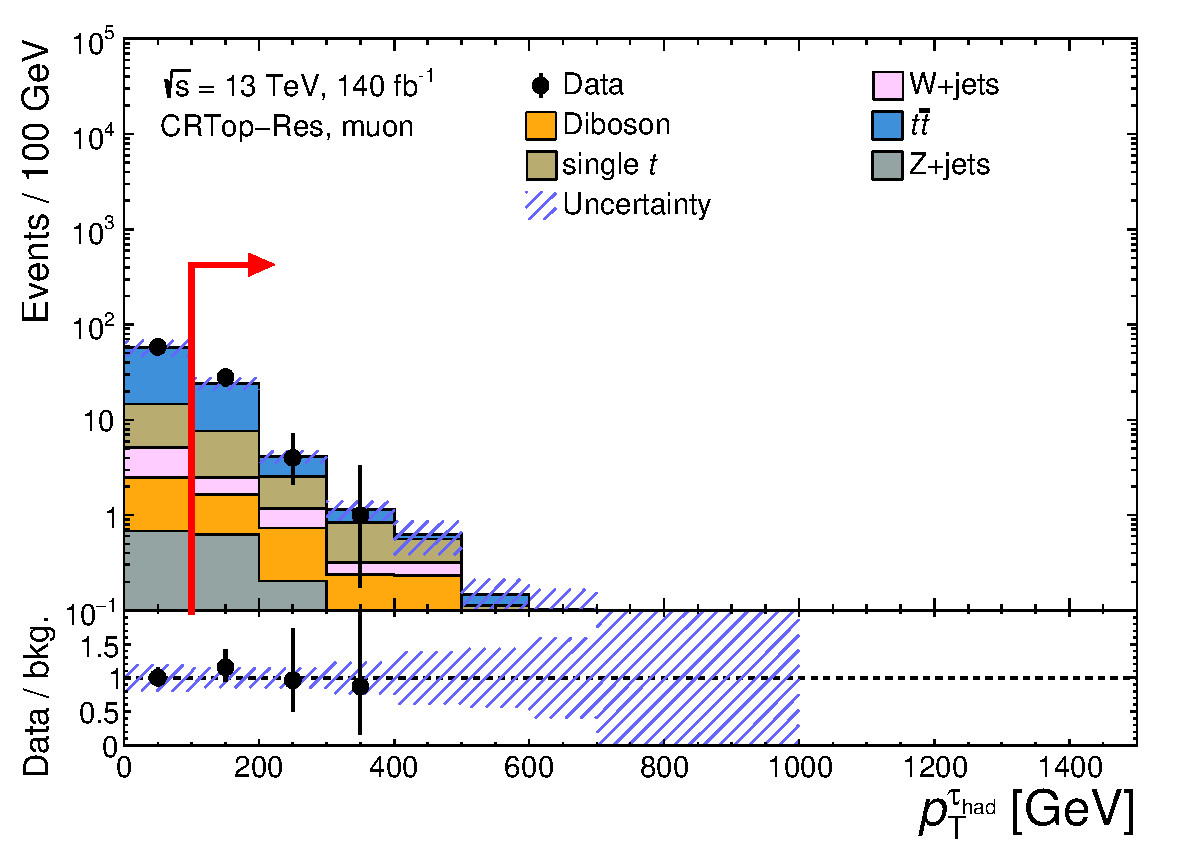
\includegraphics[width=\linewidth]{Figs/CH8/hepdata/topCR_1tau1mu_Res_tau_pT_N_minus_1_tau_pt_0.pdf}
        \caption[]{$\pT^{\hadtau}$}
    \end{subfigure}\hfill
    \begin{subfigure}{0.49\linewidth}
        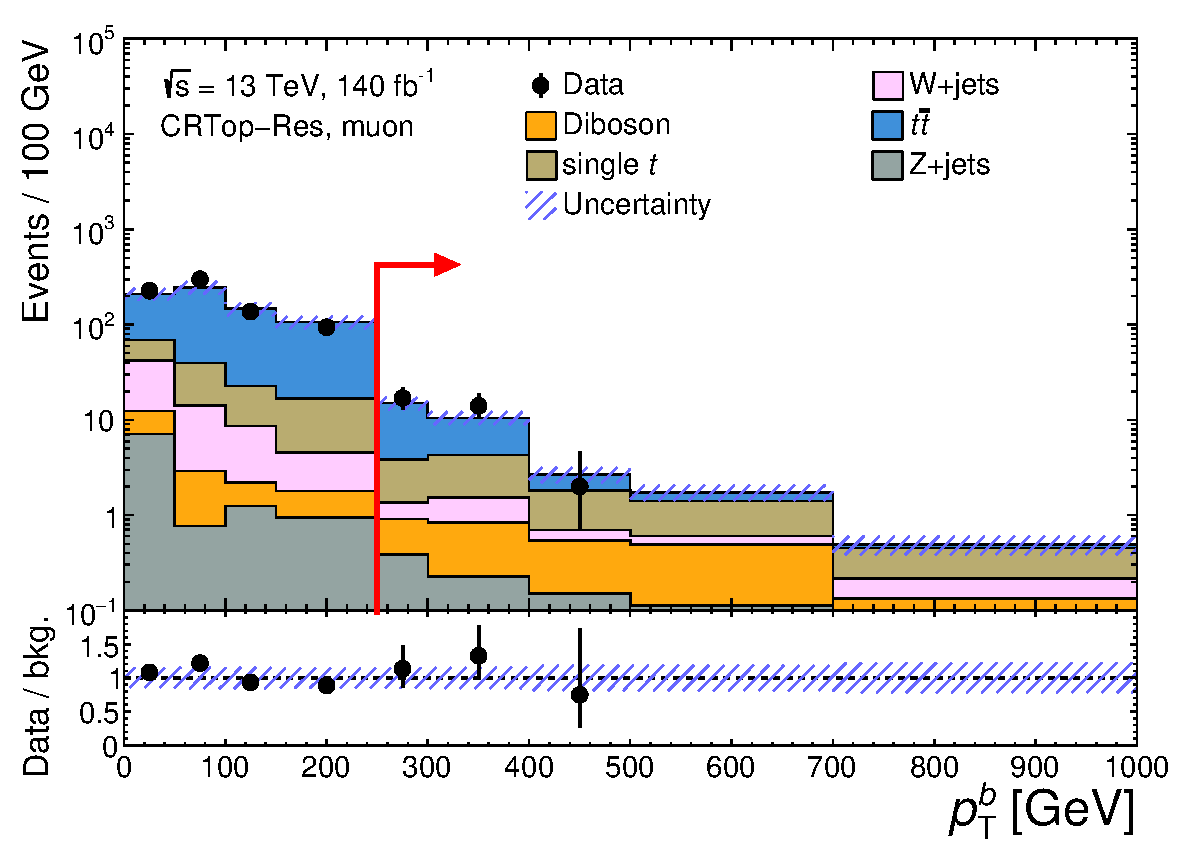
\includegraphics[width=\linewidth]{Figs/CH8/hepdata/topCR_1tau1mu_Res_bJet_pT_0_N_minus_1_bjet_pt_0.pdf}
        \caption[]{$\pT^b$}
    \end{subfigure}
% Other N-1 panels retained for reference; temporarily hidden.
%     \begin{subfigure}{0.49\linewidth}
%         \includegraphics[width=\linewidth]{Figs/CH8/hepdata/topCR_1tau1mu_Res_mT_N_minus_1_mT_tau_met.pdf}
%         \caption[]{$\mT$}
%     \end{subfigure}\hfill
%     \begin{subfigure}{0.49\linewidth}
%         \includegraphics[width=\linewidth]{Figs/CH8/hepdata/topCR_1tau1mu_Res_n_bjets_N_minus_1_n_bjets.pdf}
%         \caption[]{$N_b$}
%     \end{subfigure}
    \caption[Background-only fit distributions in CRTop-Res, muon channel]{$N-1$ distributions in $\CRTop$-$\Res$ for the $\mu$ channel after the background-only fit. The hatched bands show the combined statistical and systematic uncertainties. The bottom panels show the ratio of data to background prediction. Red arrows indicate variable thresholds for the $\CRTop$ regions. The last bin includes overflow.}
    \label{fig:ch8_topcr_res_mu}
\end{figure}

% Following figures are from /Users/zang/Desktop/fit_results/fit_taunub_sys_1l_allVR_BONLY_MU3000_gU2_5_23L1_0_noWeights_N_minus_1_fullRegion_v3_HEPData/Plots/
% Source files: topCR_1tau1e_NonRes*_postFit.eps and topCR_1tau1e_NonRes*_postfit.yaml.
% Local verified copies: data/ch8/hepdata_20260924/ (Plots, Histograms, Fits).
% Styling: scripts/ch8/restyle_hepdata.py; native data and ratio drawings are preserved.
% Verification: output/ch8/hepdata_update_20260924/figures.json.
% Axis notation/font update: scripts/ch8/axis_labels.py; output/ch8/axis_labels_20260924/.
% Previous version: figures_topcr_bonly_20260921.tex (selected by \CHEightCRFigureVersion).
\begin{figure}[htpb]
    \centering
    \begin{subfigure}{0.49\linewidth}
        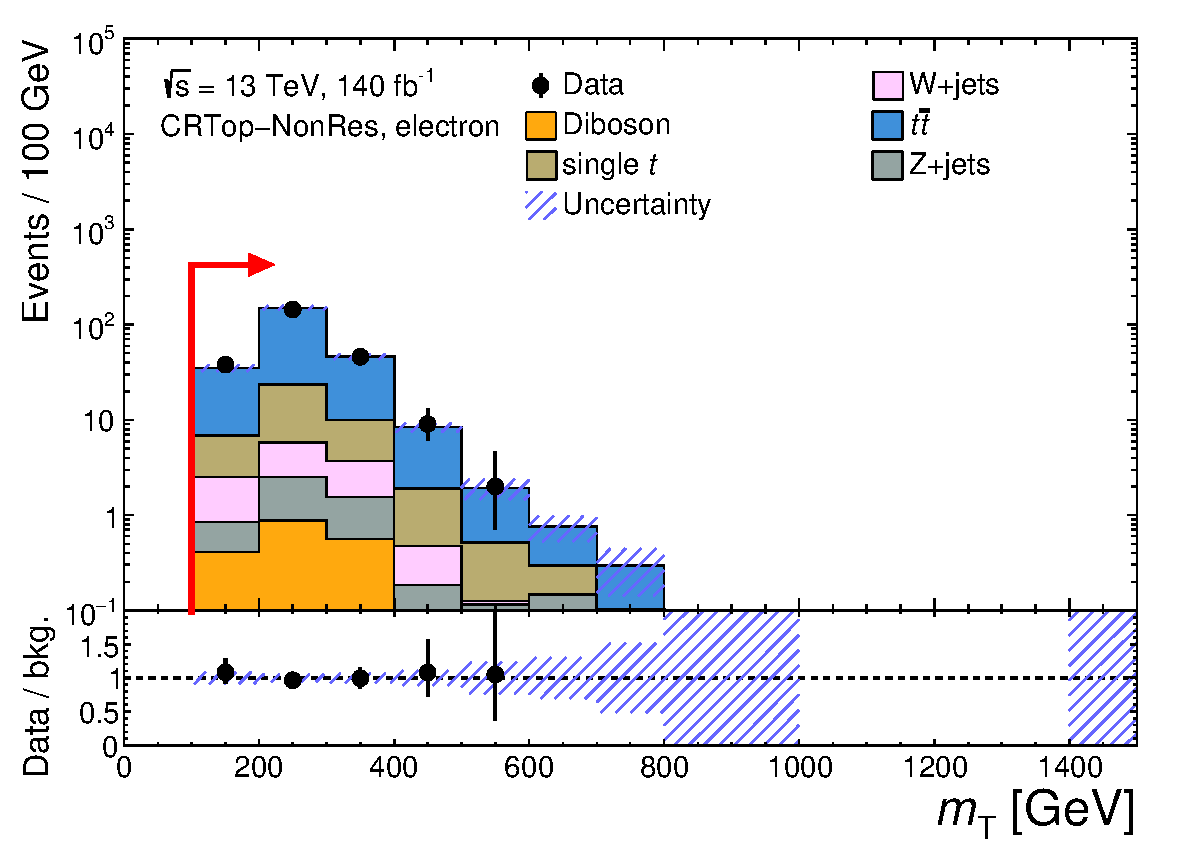
\includegraphics[width=\linewidth]{Figs/CH8/hepdata/topCR_1tau1e_NonRes_mT_N_minus_1_mT_tau_met.pdf}
        \caption[]{$\mT$}
    \end{subfigure}\hfill
    \begin{subfigure}{0.49\linewidth}
        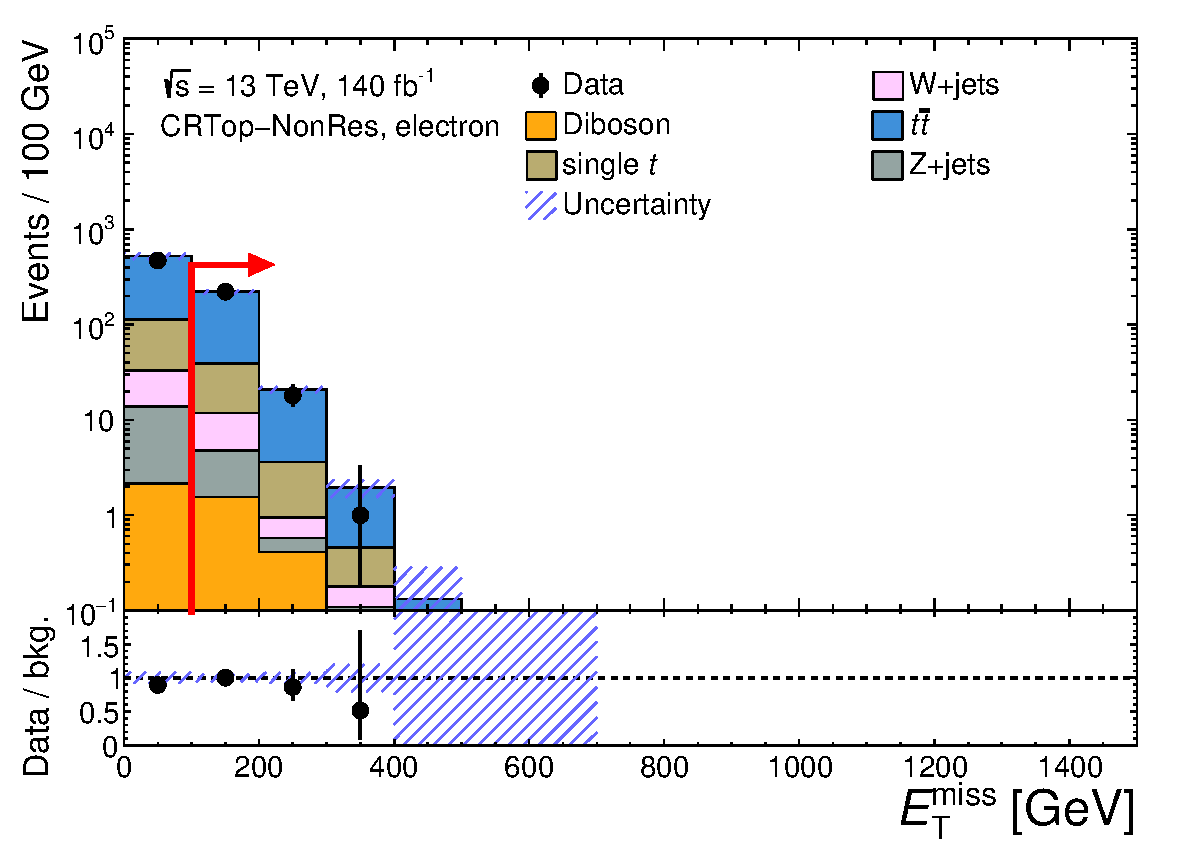
\includegraphics[width=\linewidth]{Figs/CH8/hepdata/topCR_1tau1e_NonRes_met_N_minus_1_met.pdf}
        \caption[]{$\met$}
    \end{subfigure}\\
    \begin{subfigure}{0.49\linewidth}
        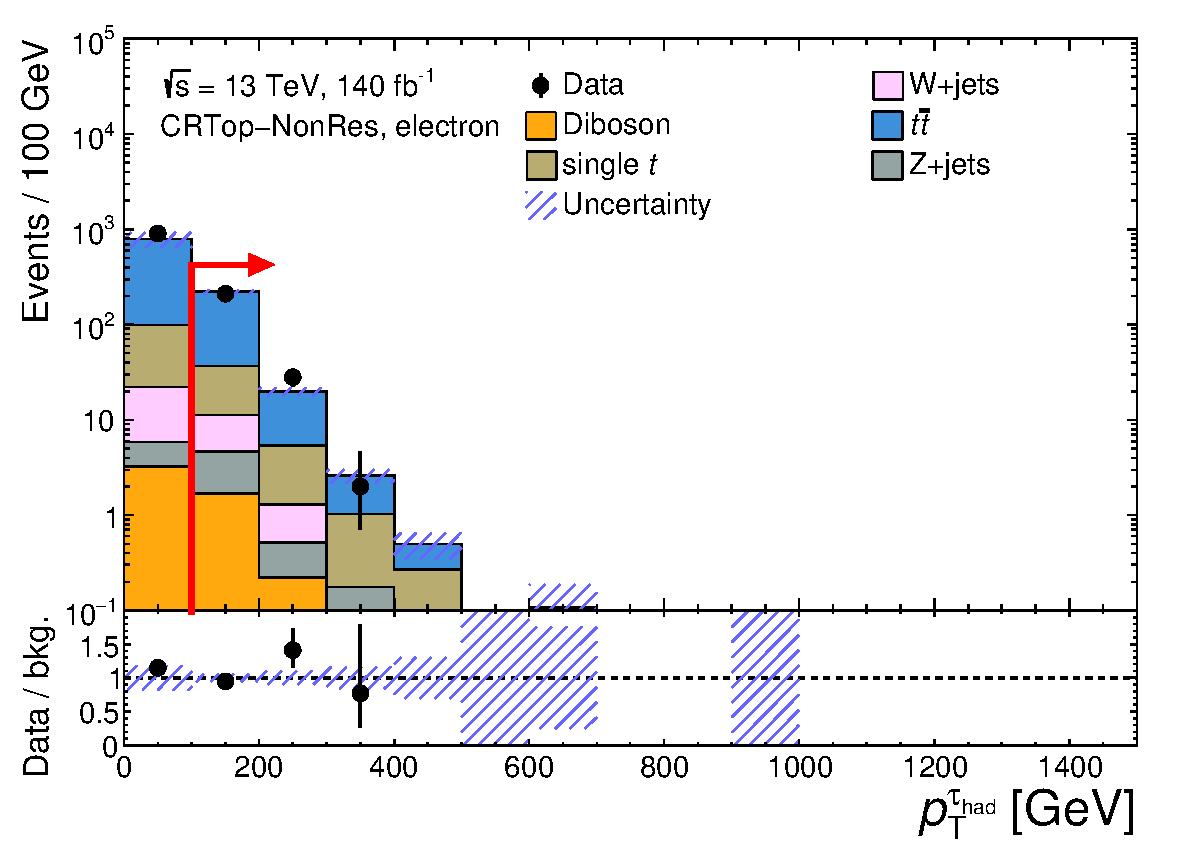
\includegraphics[width=\linewidth]{Figs/CH8/hepdata/topCR_1tau1e_NonRes_tau_pT_N_minus_1_tau_pt_0.pdf}
        \caption[]{$\pT^{\hadtau}$}
    \end{subfigure}\hfill
    \begin{subfigure}{0.49\linewidth}
        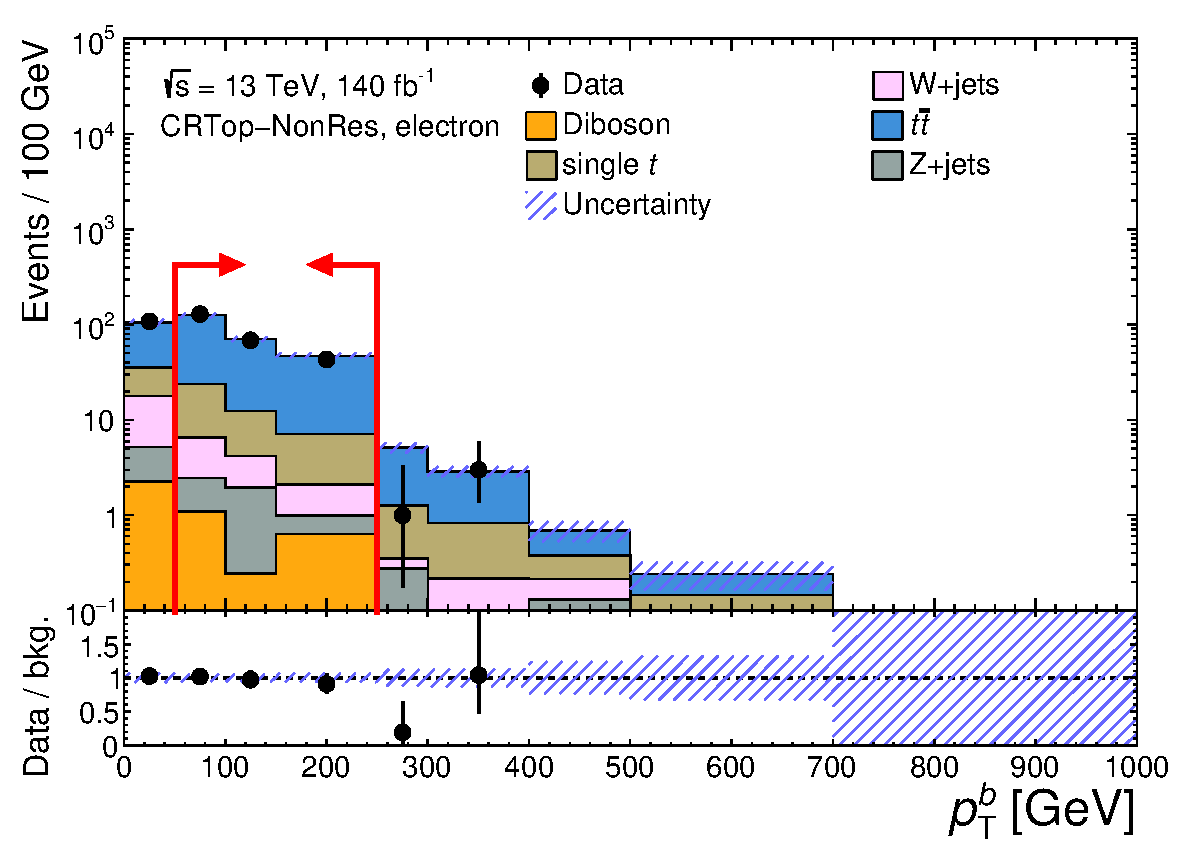
\includegraphics[width=\linewidth]{Figs/CH8/hepdata/topCR_1tau1e_NonRes_bJet_pT_0_N_minus_1_bjet_pt_0.pdf}
        \caption[]{$\pT^b$}
    \end{subfigure}
% Other N-1 panels retained for reference; temporarily hidden.
%     \begin{subfigure}{0.49\linewidth}
%         \includegraphics[width=\linewidth]{Figs/CH8/hepdata/topCR_1tau1e_NonRes_DeltaPhi_N_minus_1_dphi_taumet.pdf}
%         \caption[]{$\DphiTauMet$}
%     \end{subfigure}\hfill
%     \begin{subfigure}{0.49\linewidth}
%         \includegraphics[width=\linewidth]{Figs/CH8/hepdata/topCR_1tau1e_NonRes_n_bjets_N_minus_1_n_bjets.pdf}
%         \caption[]{$N_b$}
%     \end{subfigure}
    \caption[Background-only fit distributions in CRTop-NonRes, electron channel]{$N-1$ distributions in $\CRTop$-$\NonRes$ for the $e$ channel after the background-only fit. The hatched bands show the combined statistical and systematic uncertainties. The bottom panels show the ratio of data to background prediction. Red arrows indicate variable thresholds for the $\CRTop$ regions. The last bin includes overflow.}
    \label{fig:ch8_topcr_nonres_e}
\end{figure}

% Following figures are from /Users/zang/Desktop/fit_results/fit_taunub_sys_1l_allVR_BONLY_MU3000_gU2_5_23L1_0_noWeights_N_minus_1_fullRegion_v3_HEPData/Plots/
% Source files: topCR_1tau1mu_NonRes*_postFit.eps and topCR_1tau1mu_NonRes*_postfit.yaml.
% Local verified copies: data/ch8/hepdata_20260924/ (Plots, Histograms, Fits).
% Styling: scripts/ch8/restyle_hepdata.py; native data and ratio drawings are preserved.
% Verification: output/ch8/hepdata_update_20260924/figures.json.
% Axis notation/font update: scripts/ch8/axis_labels.py; output/ch8/axis_labels_20260924/.
% Previous version: figures_topcr_bonly_20260921.tex (selected by \CHEightCRFigureVersion).
\begin{figure}[htpb]
    \centering
    \begin{subfigure}{0.49\linewidth}
        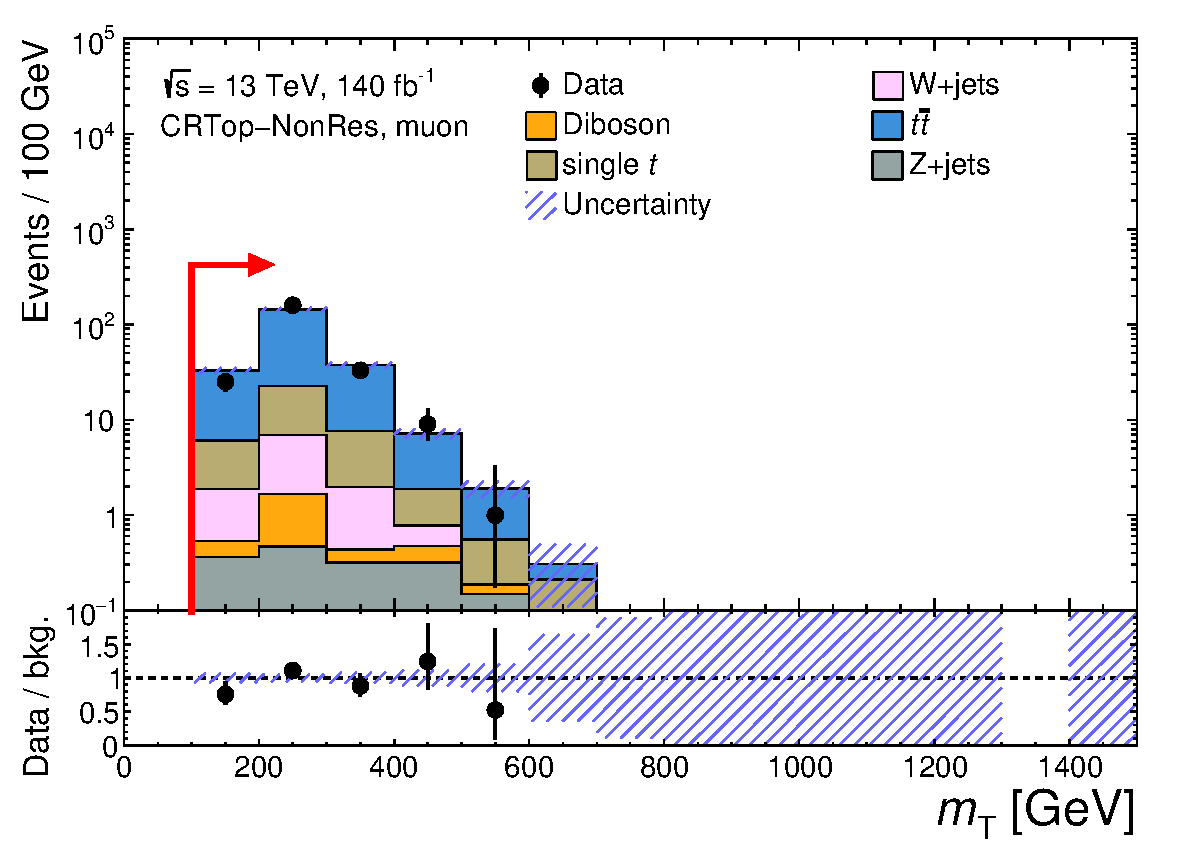
\includegraphics[width=\linewidth]{Figs/CH8/hepdata/topCR_1tau1mu_NonRes_mT_N_minus_1_mT_tau_met.pdf}
        \caption[]{$\mT$}
    \end{subfigure}\hfill
    \begin{subfigure}{0.49\linewidth}
        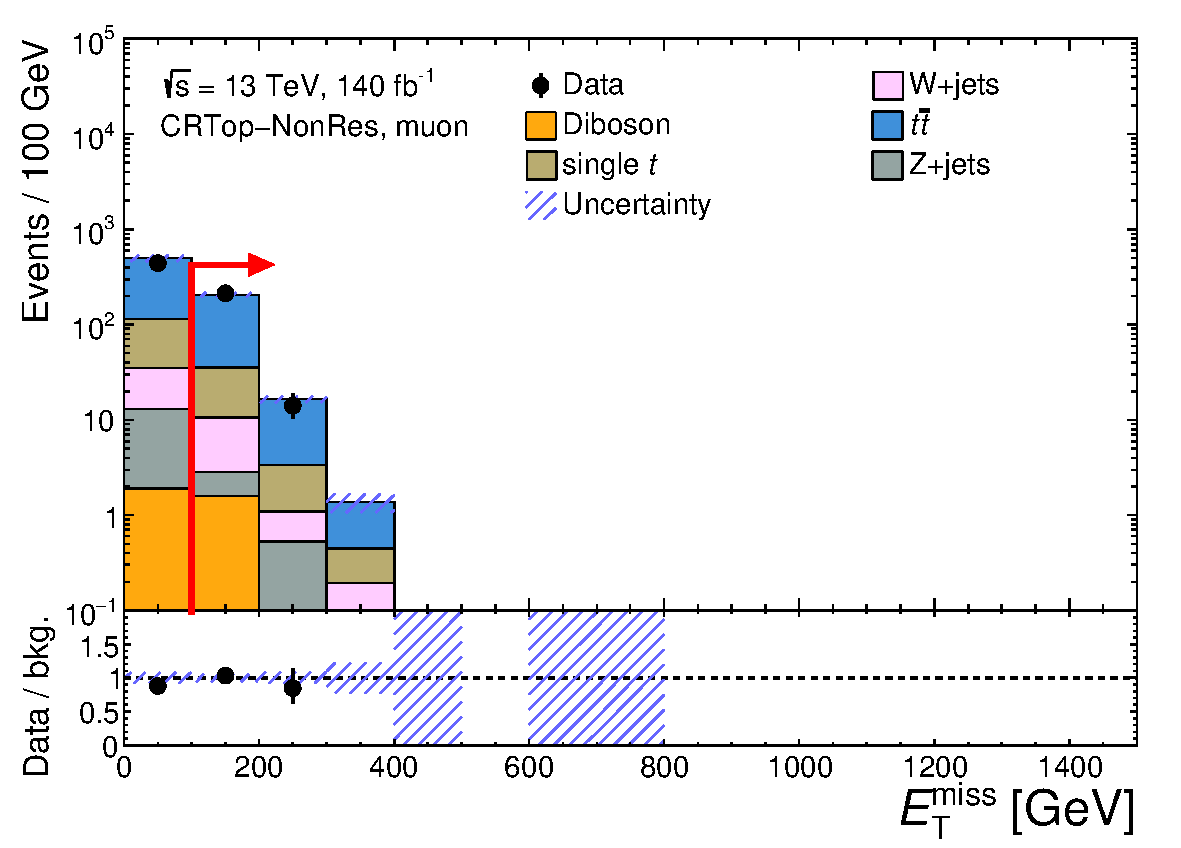
\includegraphics[width=\linewidth]{Figs/CH8/hepdata/topCR_1tau1mu_NonRes_met_N_minus_1_met.pdf}
        \caption[]{$\met$}
    \end{subfigure}\\
    \begin{subfigure}{0.49\linewidth}
        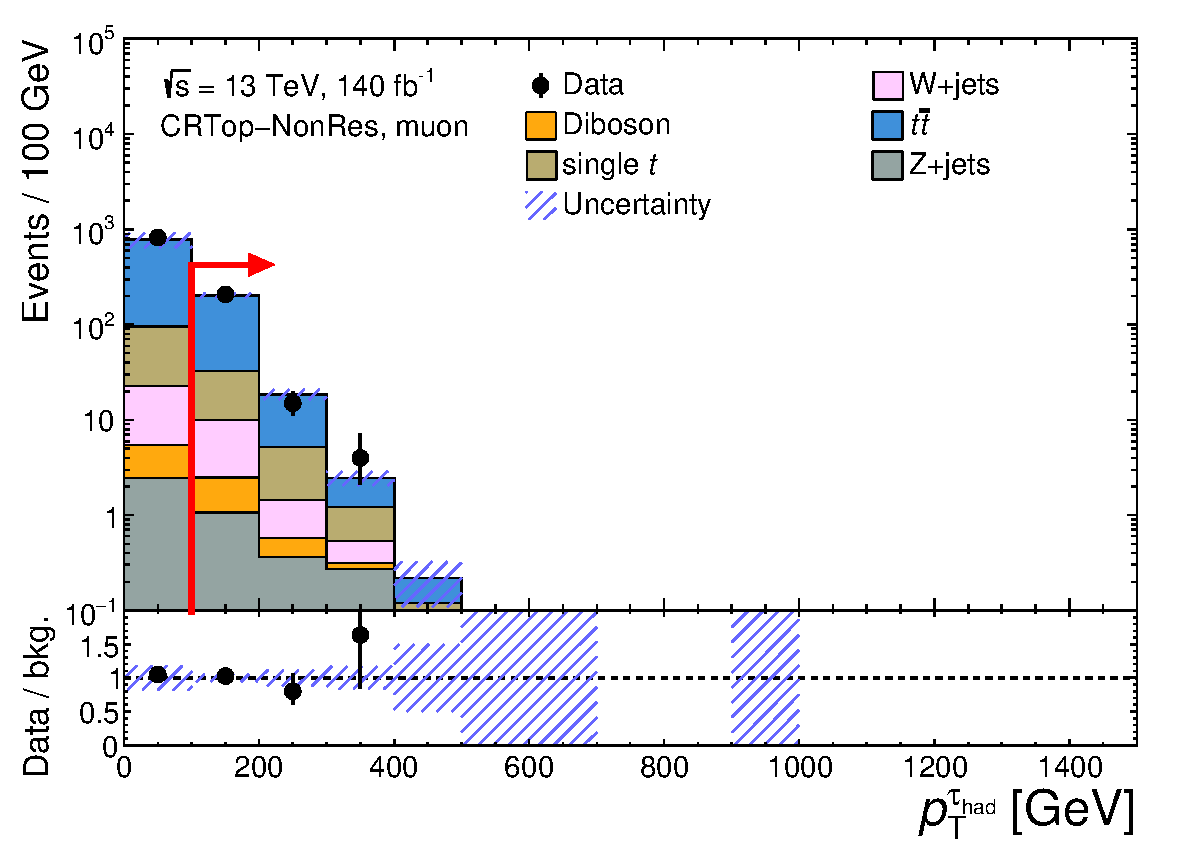
\includegraphics[width=\linewidth]{Figs/CH8/hepdata/topCR_1tau1mu_NonRes_tau_pT_N_minus_1_tau_pt_0.pdf}
        \caption[]{$\pT^{\hadtau}$}
    \end{subfigure}\hfill
    \begin{subfigure}{0.49\linewidth}
        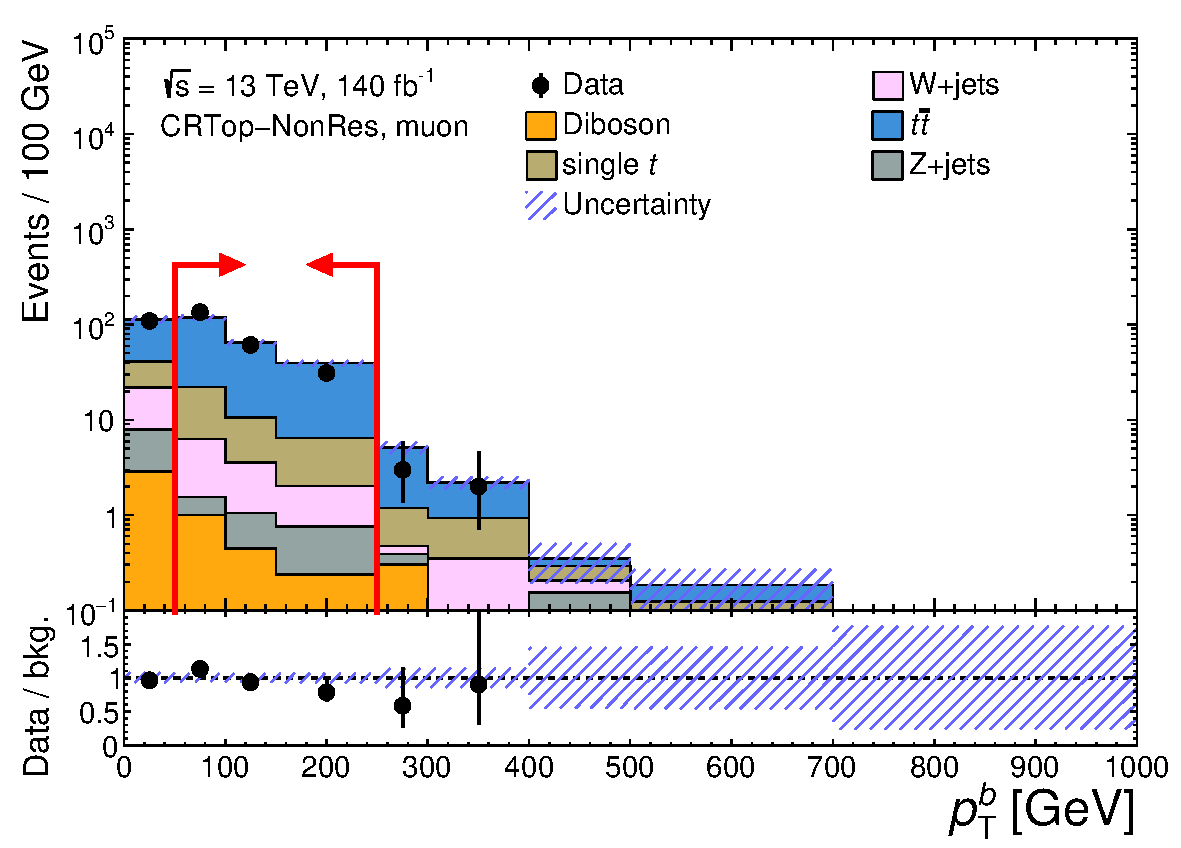
\includegraphics[width=\linewidth]{Figs/CH8/hepdata/topCR_1tau1mu_NonRes_bJet_pT_0_N_minus_1_bjet_pt_0.pdf}
        \caption[]{$\pT^b$}
    \end{subfigure}
% Other N-1 panels retained for reference; temporarily hidden.
%     \begin{subfigure}{0.49\linewidth}
%         \includegraphics[width=\linewidth]{Figs/CH8/hepdata/topCR_1tau1mu_NonRes_DeltaPhi_N_minus_1_dphi_taumet.pdf}
%         \caption[]{$\DphiTauMet$}
%     \end{subfigure}\hfill
%     \begin{subfigure}{0.49\linewidth}
%         \includegraphics[width=\linewidth]{Figs/CH8/hepdata/topCR_1tau1mu_NonRes_n_bjets_N_minus_1_n_bjets.pdf}
%         \caption[]{$N_b$}
%     \end{subfigure}
    \caption[Background-only fit distributions in CRTop-NonRes, muon channel]{$N-1$ distributions in $\CRTop$-$\NonRes$ for the $\mu$ channel after the background-only fit. The hatched bands show the combined statistical and systematic uncertainties. The bottom panels show the ratio of data to background prediction. Red arrows indicate variable thresholds for the $\CRTop$ regions. The last bin includes overflow.}
    \label{fig:ch8_topcr_nonres_mu}
\end{figure}
